\chapter{Livello di collegamento}

Nei Capitoli 2, 3 e 4 si è parlato del livello di applicazione, del livello di trasporto e del livello di rete.\
In questo capitolo parleremo invece del livello di collegamento.\
La pila dei protocolli TCP/IP non definisce alcun protocollo a livello di collegamento o fisico, in quanto questi sono argomenti di competenza delle singole reti che costituiscono Internet.\
È evidente come sul mercato ormai vi siano un gran numero di protocolli e tecnologie per il livello di collegamento.

\section{Introduzione}

Nel Capitolo 4 si è visto che la comunicazione a livello di rete avviene tra host.\
Un datagramma è un'unità dati che può essere frammentata e riassemblata ma che in generale viene inviata da un host, che si trova da qualche parte nel mondo, ad un altro host, che si trova in qualche altra zona.\
Internet non è altro che una combinazione di reti unite assieme da dispositivi di collegamento (per esempio, router e switch).\
Se un datagramma deve viaggiare da un host ad un altro, deve quindi passare necessariamente attraverso tali reti.

\subsection{Nodi e collegamenti}

Anche se la comunicazione nei livelli di applicazione, trasporto e rete è end-to-end (cioè avviene, dal punto di vista logico, dall'host iniziale a quello finale), quella a livello di collegamento è invece da nodo a nodo.\
Come si è visto nei capitoli precedenti, un'unità di dati (cioè un pacchetto) trasmessa da un certo punto della rete per arrivare fino alla sua destinazione deve attraversare molte altre reti (LAN e WAN) collegate per mezzo di router.\
È consuetudine riferirsi ai router e agli host alle due estremità come a \emph{nodi} e alle reti nel mezzo come a \emph{collegamenti}.

\begin{figure}[H]
    \centering
    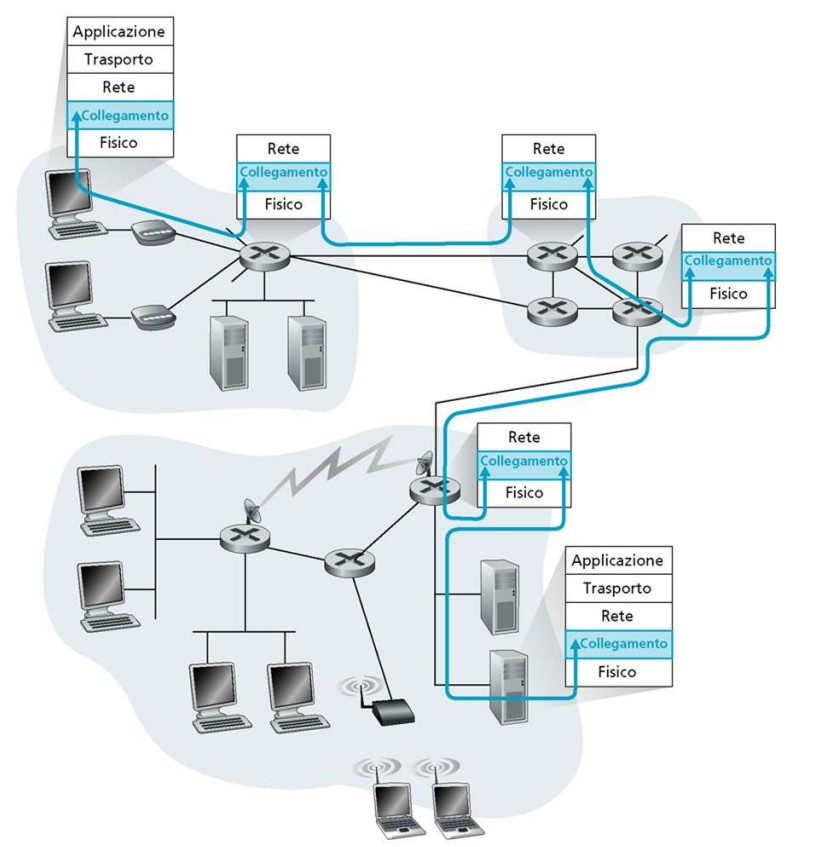
\includegraphics[width=0.7\textwidth]{immagini/Livello_Collegamento.jpg}
    \caption*{Comunicazione a livello di collegamento}
\end{figure}

\subsection{Due tipi di collegamento}

I nodi all'interno delle reti sono fisicamente collegati da un mezzo trasmissivo, come un cavo o l'aria.\
Compito del livello di collegamento è controllare come viene usato tale mezzo.\
Possiamo avere un livello di collegamento che utilizza l'intera capacità di un mezzo oppure solo una parte della sua capacità.\
In altre parole, possiamo avere un \emph{collegamento punto-punto} o un \emph{collegamento broadcast}.\
In un collegamento punto-punto, il collegamento è dedicato a due soli dispositivi (mittente e ricevente).\
Viceversa, in un collegamento broadcast, il collegamento è condiviso tra varie coppie di dispositivi.\
Per esempio, quando due amici usano il telefono di casa per chiacchierare, stanno usando un collegamento punto-punto.\
Quando gli stessi due amici usano i loro telefoni cellulari, stanno usando un collegamento broadcast (visto che l'aria viene condivisa tra vari utilizzatori di cellulari).

\subsection{Due sotto-livelli}

Per comprendere meglio le funzionalità ed i servizi forniti dal livello di collegamento possiamo dividere questo livello in due sotto-livelli:\ il \emph{Data-Link Control} (\emph{DLC}) ed il \emph{controllo dell'accesso al mezzo trasmissivo} (\emph{Media Access Control, MAC}).\
Il sotto-livello DLC si occupa di tutte le questioni comuni sia ai collegamenti punto-punto che a quelli broadcast.\
Il sotto-livello MAC si occupa invece solo degli aspetti specifici dei canali broadcast

\subsection{Servizi offerti}

\subsubsection{Framing}

Trasmettere i dati, a livello fisico, significa inviare i bit sotto forma di segnali dalla sorgente alla destinazione.\
Il livello fisico fornisce la necessaria sincronizzazione in modo che il mittente e il ricevente utilizzino la stessa durata, e temporizzazione, per i bit.

Il livello collegamento, inoltre, ha la necessità di raggruppare i bit all'interno di frame, questo per fare in modo che sia possibile stabilire un ordine tra i bit e distinguerli gli uni dagli altri.\
Il sistema postale che tutti conosciamo implementa una sorta di framing.\
Il semplice fatto di inserire una lettera in una busta separa un'informazione da un'altra:\ la busta funge da delimitatore tra le varie lettere.\
Inoltre, ogni busta riporta l'indirizzo del mittente e quello del ricevente.\
Entrambi questi indirizzi sono necessari visto che il sistema postale è un servizio di consegna molti-a-molti.

Il \emph{framing}, a livello di collegamento, ha il compito di separare i vari messaggi durante la trasmissione da una sorgente a una destinazione.\
Opera aggiungendo a singoli frame sia l'indirizzo del mittente che quello della destinazione.\
L'indirizzo di destinazione indica dove deve andare il pacchetto, quello del mittente serve invece al ricevente per poter generare un riscontro dell'avvenuta ricezione (\emph{acknowledgment}).

Anche se un intero messaggio (ad esempio di livello applicazione) potrebbe essere inserito in un unico frame, normalmente questo non avviene.\
Una ragione è che, in presenza di messaggi grandi, il frame diventerebbe molto grande, rendendo inefficienti i controlli del flusso e degli errori.\
Inoltre, il trasporto di un messaggio in un frame di grandi dimensioni avrebbe come effetto collaterale che anche l'errore su un singolo bit provocherebbe la necessità di ritrasmettere l'intero frame.\
Quando invece il messaggio viene suddiviso in frame più piccoli, l'errore su un singolo bit coinvolge solamente quel piccolo frame (che dovrà essere ritrasmesso).

\subsubsection{Consegna affidabile}

\begin{itemize}
    \item È considerata non necessaria nei collegamenti che presentano un basso numero di errori sui bit (fibra ottica, cavo coassiale e doppino intrecciato).
    \item È spesso utilizzata nei collegamenti soggetti a elevati tassi di errori (es.:\ collegamenti wireless).
\end{itemize}

\subsubsection{Controllo di flusso}

\begin{itemize}
    \item Evita che il nodo trasmittente saturi quello ricevente.
\end{itemize}

\subsubsection{Rilevazione degli errori}

\begin{itemize}
    \item Gli errori sono causati dall’attenuazione del segnale e da rumore elettromagnetico.
    \item Il nodo ricevente individua la presenza di errori:\ è possibile grazie all’inserimento, da parte del nodo trasmittente, di bit di controllo di errore all’interno del frame.
\end{itemize}

\subsubsection{Correzione degli errori}

\begin{itemize}
    \item Il nodo ricevente determina anche il punto in cui si è verificato l’errore e lo corregge
\end{itemize}

\section{Indirizzamento a livello di collegamento}

Il prossimo argomento da affrontare sono gli indirizzi di livello collegamento.\
Nel capitolo 4 si è parlato degli indirizzi IP come identificatori del livello di rete, identificatori che individuano con esattezza i punti di Internet dove sono connessi gli host sorgente e destinazione.\
Tuttavia, in una rete senza connessione come Internet non è possibile far sì che un datagramma raggiunga la sua destinazione solamente usando gli indirizzi IP.\
La ragione è che ogni datagramma in Internet, dallo stesso host sorgente allo stesso host destinazione, può prendere un percorso diverso.\
Gli indirizzi IP sorgente e destinazione definiscono le due estremità della rete, ma non dicono attraverso quali collegamenti deve passare il datagramma.

È bene anche ricordare che gli indirizzi IP in un datagramma non dovrebbero essere modificati durante il trasferimento.\
Se in un datagramma cambia l'indirizzo IP di destinazione, il pacchetto non raggiungerà la sua destinazione; se cambia quello della sorgente, l'host di destinazione o i router non potranno comunicare la risposta alla sorgente o riportare eventuali errori.

Quanto sopra indica che, in una rete senza connessione, è necessario avere un ulteriore meccanismo di indirizzamento:\ gli indirizzi di livello collegamento.\
Un \emph{indirizzo di livello collegamento} (indirizzo di collegamento, link-layer address, link address) è spesso chiamato anche indirizzo fisico oppure indirizzo MAC (MAC address).

I collegamenti sono ovviamente controllati dal livello di collegamento e utilizzano indirizzi di questo livello.\
Quando un datagramma passa dal livello di rete al livello di collegamento, esso viene racchiuso all'interno di un frame e viene aggiunta un'intestazione che contiene due indirizzi di livello collegamento (sorgente e destinazione del frame).\
Questi due indirizzi vengono cambiati ogni volta che il frame passa da un collegamento a un altro.

\subsection{Address Resolution Protocol (ARP)}

Assumiamo che su Internet ci sia un nodo che intende comunicare con un altro nodo e che questa coppia di nodi sia separata da un certo numero di router.\
Il nodo mittente ovviamente conosce l'indirizzo IP della destinazione ed inoltre è a conoscenza del router di default che si trova all'interno della sua rete locale.\
Ogni router, tranne l'ultimo, nel percorso tra sorgente e destinazione ricava l'indirizzo IP del router successivo utilizzando la tabella d'inoltro.\
L'ultimo router conosce l'indirizzo IP dell'host di destinazione.\
Tuttavia, l'indirizzo IP del nodo successivo non è sufficiente per la trasmissione di un frame attraverso un collegamento:\ è necessario avere l'indirizzo di collegamento del nodo successivo.

L'\emph{Address Resolution Protocol (ARP)} serve proprio per questo scopo.\
Il protocollo ARP è uno dei protocolli ausiliari definiti a livello di rete, come mostrato nella Figura \ref{fig:ARP}

\begin{figure}[H]
    \centering
    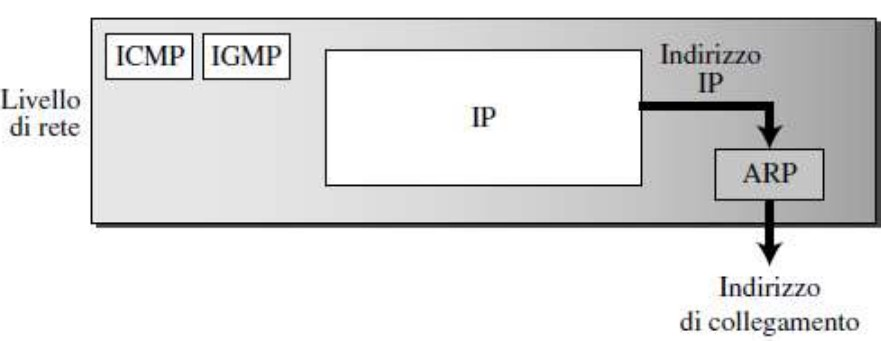
\includegraphics[width=0.7\textwidth]{immagini/ARP.jpg}
    \caption{Posizione dell'ARP nella pila TCP/IP.}
    \label{fig:ARP}
\end{figure}

Appartiene al livello di rete, ma abbiamo deciso di rimandare la sua analisi fino ad ora proprio perché il suo scopo è associare gli indirizzi IP agli indirizzi di collegamento.\
L'ARP accetta in input un indirizzo IP, individua l'indirizzo di collegamento corrispondente e lo passa al livello di collegamento.

Ogni volta che un host o un router deve trovare l'indirizzo di collegamento di un altro host o router che si trova all'interno della sua rete, invia un pacchetto di richiesta ARP che comprende l'indirizzo di collegamento, l'indirizzo IP del mittente e l'indirizzo IP del ricevente.\
Siccome il mittente non conosce ancora l'indirizzo di collegamento del ricevente, la richiesta viene trasmessa usando un broadcast a livello di collegamento.\
L'invio broadcast è ottenuto per mezzo del corrispondente indirizzo di broadcast (vedi Figura \ref{fig:Funzionamento}), in modo che la richiesta raggiunga tutti i nodi all'interno della rete locale.

Ogni host o router nella rete locale riceve ed elabora il pacchetto di richiesta ARP, ma solo il ricevente designato riconosce il suo indirizzo IP e restituisce un pacchetto di risposta ARP che contiene i suoi indirizzi IP e di collegamento.\
Il pacchetto di risposta viene inviato in modalità unicast direttamente al nodo che ha inviato la richiesta.

\begin{figure}[H]
    \centering
    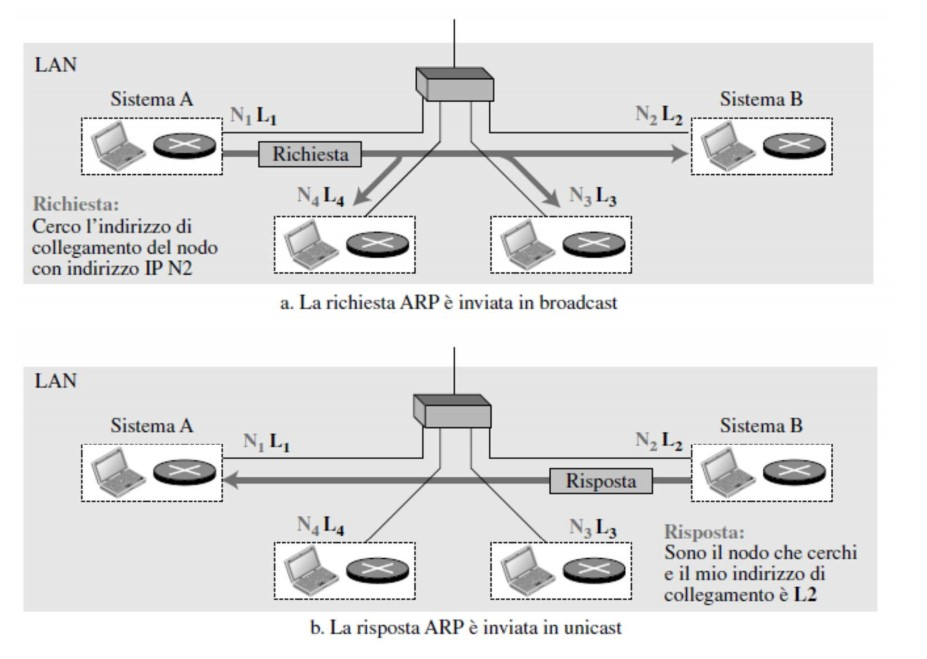
\includegraphics[width=0.8\textwidth]{immagini/ARP_funzionamento.jpg}
    \caption{Funzionamento dell'ARP}
    \label{fig:Funzionamento}
\end{figure}

\pagebreak

\subsubsection{Tabella ARP}

\begin{itemize}
    \item Ogni nodo IP (host, router) nella LAN ha una tabella ARP.
    \item Tabella ARP:\ contiene la corrispondenza tra indirizzi IP e MAC.
          \begin{itemize}
              \item $<$Indirizzo IP; Indirizzo MAC; TTL$>$
          \end{itemize}
    \item TTL (tempo di vita):\ valore che indica quando bisognerà eliminare una data voce nella tabella (il tempo di vita tipico è di 20 min)
    \item Poiché ARP risolve gli indirizzi IP solo per i nodi della stessa LAN, le tabelle ARP contengono la corrispondenza fra indirizzi IP e indirizzi MAC per i nodi della stessa sottorete.
    \item La tabella non contiene necessariamente le corrispondenze per tutti i nodi della sottorete.
\end{itemize}

\begin{figure}[H]
    \centering
    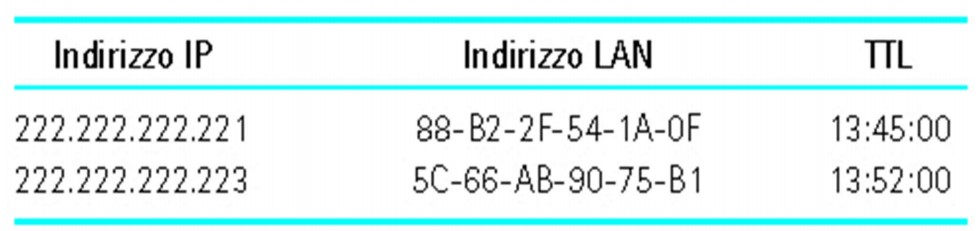
\includegraphics[width=0.7\textwidth]{immagini/ARP_Tabella.jpg}
    \caption*{Tabella ARP}
\end{figure}

\subsubsection{\emph{Formato del pacchetto ARP}}

\begin{figure}[H]
    \centering
    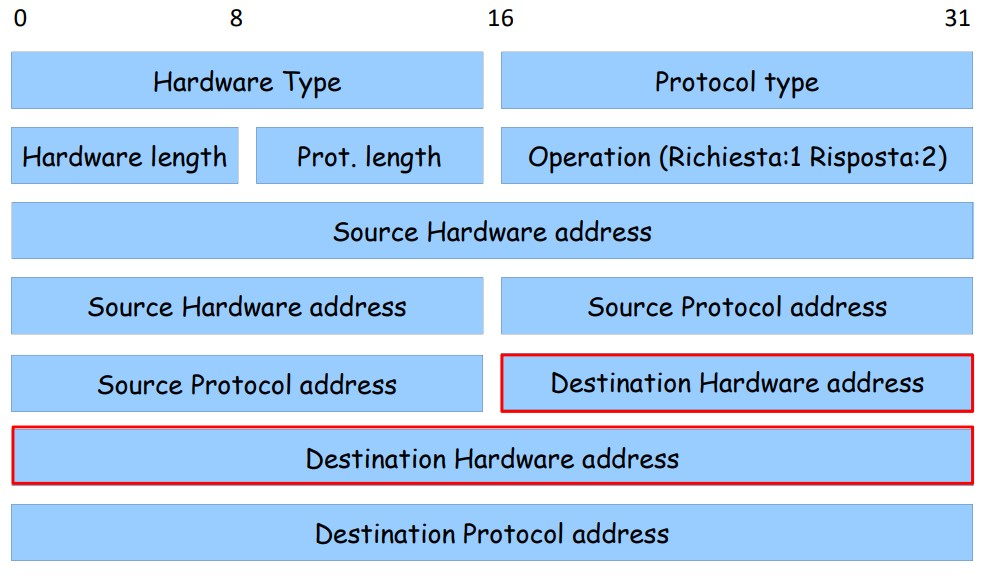
\includegraphics[width=0.8\textwidth]{immagini/Pacchetto_ARP.jpg}
    \caption*{Formato del pacchetto ARP.}
\end{figure}
Il campo \emph{hardware type} definisce il tipo del protocollo di livello collegamento che viene usato, ad Ethernet viene assegnato il tipo 1.\
Il campo \emph{protocol type} definisce il protocollo del livello di rete:\ il codice del protocollo IPv4 è (0800)\textsubscript{16}.

I campi \emph{source hardware address} e \emph{source protocol address} definiscono, per il mittente, il suo indirizzo fisico e quello del protocollo di livello superiore (IP nel nostro esempio).\
Entrambi i campi, per i motivi discussi in precedenza, sono di lunghezza variabile (lunghezze definite per mezzo di \emph{hardware lenght} e \emph{protocol lenght}).\
I campi \emph{destination hardware address} e \emph{destination protocol address} definiscono l'indirizzo fisico e quello del protocollo di livello superiore, ma in questo caso per il ricevente.\
I pacchetti ARP vengono incapsulati direttamente all'interno dei frame di livello collegamento.\
Per questo motivo il frame dovrà indicare all'interno della sua intestazione che trasporta un pacchetto ARP invece di un datagramma del livello di rete.

\subsubsection{Forwarding diretto/indiretto}

\textbf{Forwarding diretto}:\ vedi Figura \ref{fig:Funzionamento}\\
\textbf{Forwarding indiretto}:\ invio di un datagramma con mittente IP di A e destinatario IP di B.\
Ipotesi:
\begin{itemize}
    \item A conosce l’indirizzo IP di B
    \item A conosce l’indirizzo IP del primo router $\rightarrow$ DHCP
    \item A conosce l’indirizzo MAC di R $\rightarrow$ ARP
\end{itemize}
\begin{enumerate}
    \item A crea un datagramma IP con IP sorgente A, destinazione B
          \begin{enumerate}
              \item A crea un frame con indirizzo MAC destinazione il MAC address di R, il frame incapsula il datagramma IP (A-to-B)
          \end{enumerate}
    \item frame inviato da A a R
    \item frame ricevuto da R, decapsulato, il datagramma passa al livello IP
          \begin{enumerate}
              \item R estrae il datagramma IP dal frame Ethernet, e vede che la sua destinazione è B.
              \item R usa ARP per ottenere l’indirizzo MAC di B
              \item R crea un frame con destinazione il MAC address di B
          \end{enumerate}
    \item R inoltra il datagramma con IP sorgente A, destinazione B
\end{enumerate}

\section{LAN cablate:\ protocollo Ethernet}

\subsection{Progetto IEEE 802}

Abbiamo iniziato a parlare del protocollo Ethernet e delle sue varie generazioni.\
Prima di approfondire in dettaglio le sue caratteristiche è però necessario parlare brevemente dello standard IEEE che viene spesso citato nei documenti tecnici.\
Nel 1985, la IEEE Computer Society (Institute of Electrical and Electronics Engineers) iniziò un progetto, chiamato \emph{Progetto 802}, con l'obiettivo di definire uno standard per l'interconnessione tra dispositivi di produttori differenti.\
Il Progetto 802 non aveva lo scopo di sostituire una qualsiasi parte del modello OSI o la pila TCP/IP, ma piuttosto intendeva definire chiaramente le funzioni specifiche del livello fisico e di collegamento dei protocolli LAN.\
Questo lavoro ha portato alla definizione dell'IEEE Standard 802.

\subsection{Ethernet Standard}

In questa parte del testo si fa riferimento alla tecnologia Ethernet originale con velocità di trasferimento dei dati a 10 Mbps (Ethernet Standard).\
Nonostante l'evoluzione di Ethernet abbia portato a molti cambiamenti nei meccanismi utilizzati, alcune caratteristiche sono rimaste invariate nel corso dell'evoluzione.\
Parliamo quindi della versione standard per comprendere meglio le versioni successive.

\subsubsection{\emph{Formato dei frame}}

Il frame Ethernet contiene sei campi, come mostrato nella Figura \ref{fig:Frame}.

\begin{figure}[H]
    \centering
    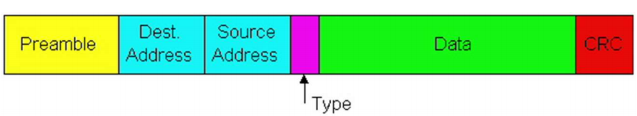
\includegraphics[width=0.8\textwidth]{immagini/Frame_Ethernet.png}
    \caption{Struttura dei frame Ethernet.}
    \label{fig:Frame}
\end{figure}

\begin{itemize}
    \item \textbf{\emph{Preamble} (\emph{preambolo})}.\
          I pacchetti Ethernet iniziano con un campo di otto byte:\ sette hanno i bit 10101010 e l’ultimo è 10101011.\
          Servono per ``attivare'' gli adattatori dei riceventi e sincronizzare i loro orologi con quello del trasmittente.
    \item \textbf{\emph{Destination Address} (\emph{DA, Indirizzo di destinazione})}.\
          Il campo (6 byte quindi 48) contiene l'indirizzo di collegamento della stazione o delle stazioni destinatarie del frame.\
          Quando la stazione ricevente trova in questo campo il suo stesso indirizzo di livello collegamento (unicast), l'indirizzo multicast di un gruppo di cui fa parte, o l'indirizzo broadcast, estrae i dati dal frame e li passa al protocollo di livello superiore (definito dal valore del campo Type).
    \item \textbf{\emph{Source Address} (\emph{SA, Indirizzo della sorgente})}.\
          Anche questo campo è di 6 byte e contiene l'indirizzo di collegamento del mittente del frame.
    \item \textbf{\emph{Type} (\emph{Type})}.\
          Questo campo definisce il protocollo di livello superiore del pacchetto incapsulato all'interno del frame.\
          Il protocollo può essere IP, ARP, e così via.\
          In altre parole, ha lo stesso scopo del campo protocollo nell'intestazione dei datagrammmi e del numero di porta in un segmento TCP o in un datagramma utente (UDP).\
          È quindi necessario per il multiplexing e il demultiplexing a livello di collegamento.
    \item \textbf{\emph{Data and padding} (\emph{Dati})}.\
          Questo campo trasporta i dati incapsulati nel frame dai protocolli di livello superiore.\
          Ha un minimo di 46 byte e un massimo di 1500 byte.\
          Se i dati che provengono dal livello superiore superano i 1500 byte, essi devono essere frammentati e quindi racchiusi in più frame.\
          Se sono meno di 46 byte, è necessario aggiungere tanti 0 quanti sono necessari per arrivare alla dimensione minima (\emph{padding}).\
          Una volta decapsulati i dati contenuti nel frame vengono consegnati così come sono al protocollo di livello superiore, quindi senza rimuovere il padding (gli 0 aggiuntivi).\
          Ciò significa che la rimozione o l'aggiunta del padding è responsabilità del livello superiore.\
          Questo obbliga il protocollo di livello superiore a conoscere la vera lunghezza dei dati inviati, in caso contrario non sarebbe in grado di distinguere i suoi dati dagli 0 aggiuntivi.\
          Proprio per questo motivo, nell'intestazione dei datagrammi è presente un campo che definisce la dimensione dei dati contenuti nel payload del datagramma.
    \item\textbf{\emph{CRC}}.\
          L'ultimo campo contiene informazioni per il rilevamento errori.\
          Il codice di ridondanza contenuto in questo campo viene calcolato sui campi indirizzo, tipo e dati.\
          Se il ricevente lo calcola e constata che non è 0, allora il frame è stato alterato durante la trasmissione, e quindi il ricevente si limita a scartarlo.
\end{itemize}

\subsubsection{\emph{Servizio senza connessione e inaffidabile}}

Ethernet fornisce un servizio senza connessione, questo significa che ogni frame inviato è indipendente dal frame precedente e dal successivo.\
In Ethernet non c'è alcuna fase di apertura o chiusura della connessione, il mittente si limita ad inviare un frame ogni volta che ne ha uno pronto, indipendentemente dal fatto che il destinatario sia pronto o meno a riceverlo.\
Può accadere che il mittente sommerga il ricevente di frame, con il risultato che alcuni di questi vengano scartati.\
Nel caso in cui un frame venga scartato, il mittente non viene informato dell'accaduto.\
Dato che il protocollo IP, che usa i servizi offerti da Ethernet, è anch'esso un protocollo non affidabile e senza connsessione, anche IP non verrà a conoscenza della perdita di dati.\
Se anche il protocollo di trasporto è non affidabile e senza connessione (ad esempio UDP), solamente il livello di applicazione potrà accorgersi della perdita ed eventualmente porvi rimedio.\
Se, invece, a livello trasporto viene usato TCP, il mittente non riceverà alcun riscontro per il segmento contenuto nel frame perso e quindi lo invierà di nuovo.

L'inaffidabilità di Ethernet è pari a quella di IP e UDP.\
Se un frame viene danneggiato durante la trasmissione e il ricevente riscontra il danneggiamento (grazie al codice di ridondanza contenuto nell'intestazione del frame), il ricevente si limiterà a scartare il frame, senza alcun'altra azione.\
È dovere dei protocolli di livello superiore riscontrare la perdita dei dati e porvi rimedio.

\subsubsection{\emph{Indirizzo}}

Tutte le stazioni che fanno parte di una rete Ethernet (ad esempio un computer, una postazione di lavoro o una stampante) sono dotate di una \emph{Network Interface Card} (\emph{NIC}), comunemente detta \emph{scheda di rete}.\
La NIC viene installata nella stazione e fornisce un suo indirizzo di livello collegamento.\
Gli indirizzi Ethernet sono composti da 6 byte (48 bit) e vengono normalmente scritti in notazione esadecimale, con i due punti a dividere i vari byte.\
Ad esempio quello che segue è un indirizzo MAC Ethernet
\begin{center}
    \textbf{4A:30:10:21:10:1A}
\end{center}

\begin{center}
    \emph{Come viene garantita l’univocità?}
\end{center}
\begin{itemize}
    \item IEEE definisce ed assegna i primi 24 bit (\emph{OUI – Organization Unique Identifier}), mentre i rimanenti 24 bit vengono gestiti dalle aziende ed assegnati a livello locale.
    \item Quando una società vuole costruire adattatori, compra un blocco dispazio di  indirizzi (univocità degli indirizzi).
\end{itemize}

\subsubsection{\emph{Indirizzi unicast, multicast e broadcast}}

Un indirizzo sorgente è sempre un \emph{indirizzo unicast}, poiché il frame proviene da una sola stazione.\
Tuttavia, l'indirizzo di destinazione può essere \emph{unicast}, \emph{multicast} o \emph{broadcast}.\
Se il bit meno significativo del primo byte nell'indirizzo di destinazione è 0 allora l'indirizzo è unicast, in caso contrario è multicast.

L'indirizzo broadcast è un caso particolare dell'indirizzo multicast:\ i destinatari sono tutte le stazioni che si trovano all'interno della LAN.\
Un indirizzo di destinazione broadcast è formato solamente da 1 (cioè 48 bit impostati a 1).

\subsubsection{\emph{Distinzione tra trasmissione unicast, multicast e broadcast}}

La tecnologia Ethernet Standard utilizza un cavo coassiale (topologia bus) o una serie di doppini intrecciati (cioè coppie di cavi di rame intrecciati).\
La topologia della rete prevede un hub al centro della stella.

Nell'Ethernet Standard la trasmissione è sempre broadcast, indipendente dal fatto che si tratti di frame con destinazione unicast, multicast o broadcast.\
Nella topologia a bus, quando la stazione A invia un frame alla stazione B, tutte le stazioni lo ricevono.\
Nella topologia a stella, quando la stazione A invia un frame alla stazione B, lo riceverà l'hub.\
Siccome gli hub sono apparati del tutto passivi, non verificano l'indirizzo di destinazione del frame, ma si limitano a rigenerare il segnale dei bit e a reinviare il frame a tutte le stazioni, ad eccezione di quella da cui l'hanno ricevuto (in questo caso A).

Unicast, multicast e broadcast sono trattati diversamente dai riceventi:
\begin{itemize}
    \item in una trasmissione unicast, tutte le stazioni ricevono il frame.\
          Il destinatario designato lo memorizza e lo gestisce, tutte le altre stazioni lo scartano;
    \item in una trasmissione multicast, tutte le stazioni ricevono il frame.\
          Quelle che appartengono al gruppo multicast lo memorizzano e lo gestiscono, tutte le altre stazioni lo scartano;
    \item in una trasmissione broadcast, tutte le stazioni (eccetto il mittente) ricevono il frame, lo memorizzano e lo gestiscono.
\end{itemize}

\subsection{Fast Ethernet}

\begin{itemize}
    \item 100 Mbps
    \item Mantiene intatti formato e dimensione min/max frame
    \item Dimensione minima immutata e trasmissione 10 volte più veloce $\rightarrow$ rete più corta, due soluzioni
          \begin{itemize}
              \item Topologia a bus $\rightarrow$ hub passivo con topologia a stella e dimensione massima rete 250m (anziché 2500m)
              \item Usare un commutatore (switch) a livello link, dotato di buffer, e una connessione full-duplex per ogni host $\rightarrow$ \textbf{no collisioni}
          \end{itemize}
\end{itemize}

\subsection{Gigabit Ethernet (802.3z)}

\begin{itemize}
    \item 1000 Mbps = 1 Gbps
    \item Mantiene invariata lunghezza min/max frame
    \item Switch al centro della stella, tutti i nodi collegati ai rami della stella $\rightarrow$ \textbf{no collisioni}
\end{itemize}

\section{Dispositivi di interconnessione}

È raro trovare degli host e delle reti che operano in maniera isolata; è molto più comune utilizzare dei dispositivi di interconnessione per collegare gli host e creare una rete, e per collegare le reti tra di loro creando una internet.\
A questo scopo vengono usati i dispositivi di interconnessione, dispositivi che possono operare a diversi livelli della pila dei protocolli Internet.\
In questo testo si vedranno tre tipi di \emph{dispositivi di interconnessione}:\ i repeater (ripetitori) o hub, gli switch di livello collegamento (detti anche switch di livello 2) e i router (detti anche switch di livello 3).\
I repeater e gli hub operano solo al primo livello, il più basso, della pila dei protocolli.\
Gli switch di livello collegamento operano ai primi due livelli, ed infine, i router operano sui primi tre livelli della pila.

\subsection{Repeater e hub}

Un \emph{repeater} è un dispositivo che opera soltanto a livello fisico.\
I segnali che trasportano informazioni all'interno di una rete possono viaggiare per una distanza ben definita prima che l'attenuazione del segnale metta a repentaglio l'integrità dei dati.\
Un repeater riceve un segnale e, prima che esso diventi troppo debole o danneggiato, \emph{rigenera} e \emph{risincronizza} la sequenza di bit originale.\
Successivamente il repeater invia il segnale rigenerato.\
In passato, quando le LAN Ethernet utilizzavano la topologia a bus, si usava un repeater per collegare tra loro due segmenti di una LAN e quindi superare i limiti di lunghezza del cavo coassiale.\
Oggi le LAN Ethernet usano la topologia stella, e in questo caso il repeater è un dispositivo multi-porta (spesso chiamato \emph{hub}) che può essere utilizzato per l'interconnessione delle varie stazioni collegate e allo stesso tempo fungere da ripetitore.\
La Figura \ref{fig:Repeater} mostra che quando un frame proveniente dalla stazione A e destinato alla stazione B arriva all'hub, il segnale che rappresenta il frame viene rigenerato per evitare la presenza di segnali di disturbo possano danneggiare il frame.\
Inoltre, l'hub inoltra il frame attraverso tutte le sue porte in uscita eccetto quella da cui ha ricevuto il segnale.\
In altre parole, il frame viene trasmesso in broadcast.\
Tutte le stazioni nella LAN ricevono il frame, ma soltanto la stazione B lo memorizza mentre tutte le altre lo scartano.\
La Figura \ref{fig:Repeater} mostra il ruolo di un repeater o di un hub in una LAN commutata.

La figura mostra chiaramente che un hub non ha alcuna capacità di filtraggio, non è abbastanza intelligente da capire attraverso quale porta il frame debba essere inviato.

\begin{center}
    Un repeater non ha capacità di filtraggio.
\end{center}

Gli hub ed i repeater sono dispositivi che operano a livello fisico.\
Essi quindi non hanno indirizzi di livello collegamento e non effettuano alcuna verifica sugli indirizzi di collegamento presenti nell'intestazione dei frame che ricevono.\
Rigenerano solamente i frame ricevuti e li inviano attraverso ogni porta.

\begin{figure}[H]
    \centering
    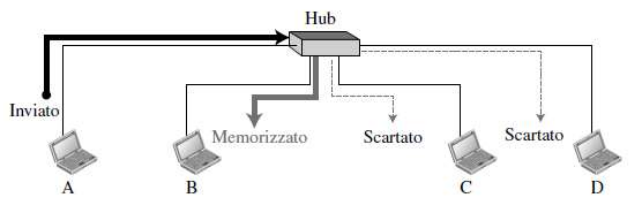
\includegraphics[width=0.8\textwidth]{immagini/Repeater.png}
    \caption{Repeater o hub}
    \label{fig:Repeater}
\end{figure}

\subsection{Switch di livello collegamento}

Uno \emph{switch di livello collegamento} (commutatore di livello collegamento) opera sia a livello fisico che a livello di collegamento.\
Come dispositivo di livello fisico rigenera il segnale che riceve.\
Inoltre, come dispositivo di livello collegamento, è in grado di verificare gli indirizzi MAC (sorgente e destinazione) contenuti nel frame.

\subsubsection{\emph{Filtraggio}}

È normale chiedersi qual è la differenza di funzionalità tra uno switch e un hub.\
Il primo ha capacità di \emph{filtraggio} (\emph{filtering}), è in grado di verificare l'indirizzo di destinazione del frame e decidere da quale porta in uscita deve essere inviato il frame.

\begin{center}
    Uno switch ha una tabella che viene utilizzata per il filtraggio.
\end{center}
\begin{figure}[H]
    \centering
    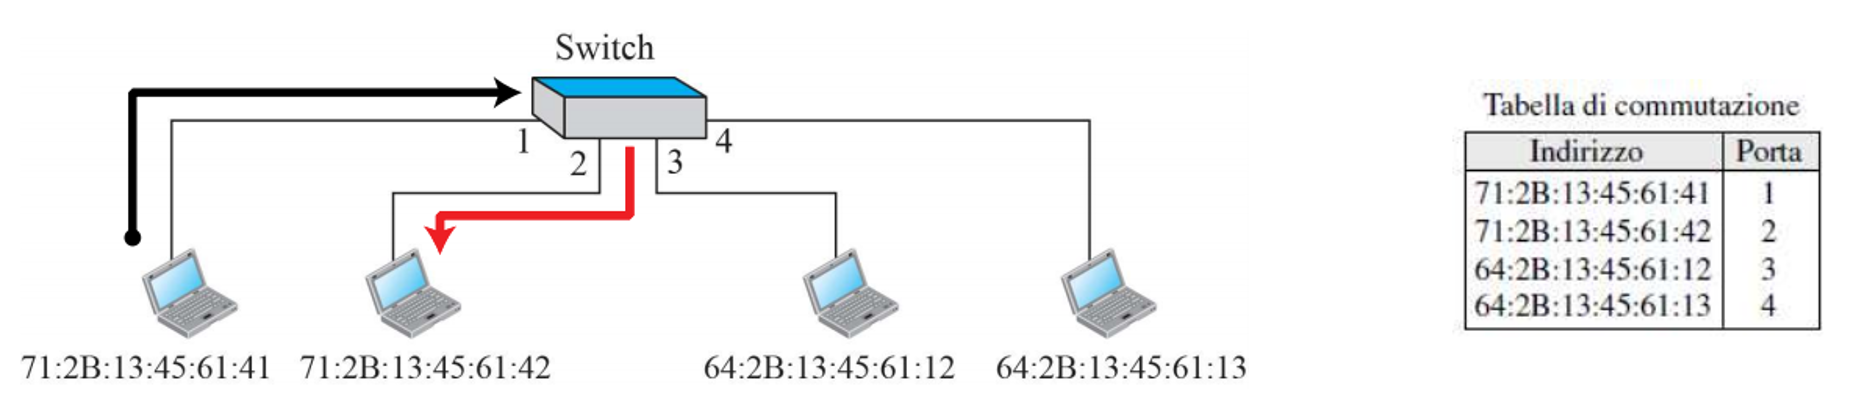
\includegraphics[width=\textwidth]{immagini/Switch.png}
    \caption{Switch di livello collegamento}
    \label{fig:Switch}
\end{figure}
Vediamo un esempio, nella Figura \ref{fig:Switch} c'è una LAN con quattro stazioni connesse a uno switch.\
Se un frame destinato alla stazione 71:2B:13:45:61:42 arriva alla porta \textbf{1}, lo switch consulta la sua tabella per individuare la porta da cui inviarlo.

Secondo la sua tabella, i frame destinati a 71:2B:13:45:61:42 devono essere inviati solo attraverso la porta 2 e quindi non è necessario inoltrare il frame attraverso altre porte.

\begin{center}
    Uno switch non modifica gli indirizzi MAC contenuti nell'intestazione dei frame.
\end{center}

\subsubsection{\emph{Switch trasparenti}}

Uno \emph{switch trasparente} è un commutatore di cui le stazioni presenti nella rete sono completamente ignare dell'esistenza del dispositivo di rete.\
Se uno switch viene aggiunto o eliminato dalla rete, non è necessaria alcuna operazione di riconfigurazione delle stazioni.\
Secondo quanto specificato nello standard IEEE 802.1, una rete dotata di switch trasparenti deve soddisfare tre criteri:
\begin{itemize}
    \item deve essere possibile inoltrare i frame da una stazione ad un'altra;
    \item la tabella d'inoltro deve essere creata automaticamente analizzando i frame che vengono spediti nella rete;
    \item devono essere evitati cicli nella rete.
\end{itemize}

\paragraph{\emph{Inoltro}}

Nel caso di uno switch trasparente l'inoltro dei frame non subisce alcuna modifica, è esattamente come descritto in precedenza.

\paragraph{\emph{Apprendimento}}

Inizialmente gli switch operavano usando delle tabelle statiche di commutazione.\
Questo significa che l'amministratore di rete era costretto ad inserire manualmente ciascuna voce della tabella durante la configurazione dello switch.\
Nonostante il processo fosse abbastanza semplice, non era molto comodo.\
Infatti, se una stazione veniva aggiunta o cancellata, la tabella doveva essere modificata manualmente.\
La stessa cosa doveva essere fatta se l'indirizzo MAC di una stazione cambiava, un evento tutt'altro che raro (ad esempio per il cambio di una scheda di rete).
\begin{figure}[H]
    \centering
    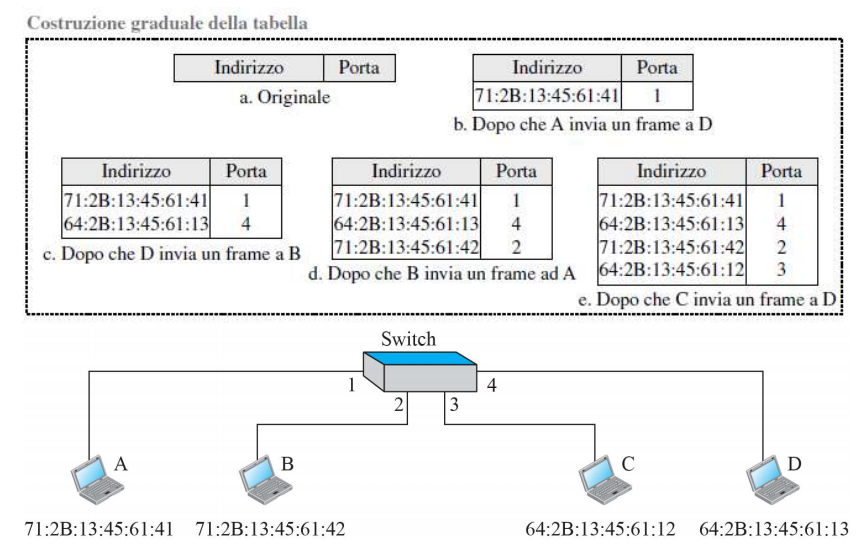
\includegraphics[width=0.8\textwidth]{immagini/Switch_autoapprendimento.png}
    \caption{Switch con auto-apprendimento}
    \label{fig:Auto-apprendimento}
\end{figure}

La soluzione, molto migliore della tabella statica, è una tabella dinamica che associa automaticamente gli indirizzi MAC alle porte (interfacce).\
Per creare una tabella dinamica, occorre uno switch che sia in grado di apprendere gradualmente dai frame che vengono inviati all'interno della rete.\
Per fare questo, lo switch analizza gli indirizzi sorgente e destinazione di ogni frame.\
L'indirizzo di destinazione viene utilizzato per decidere su quale interfaccia inoltrare il frame, quello sorgente invece serve per aggiungere nuove voci alla tabella e quindi, poco alla volta, configurarla automaticamente.\
Vediamo più in dettaglio questo procedimento utilizzando l'esempio della Figura \ref{fig:Auto-apprendimento}.

\begin{enumerate}
    \item Quando la stazione A invia un frame alla stazione D, lo switch nella sua tabella non ha alcuna voce sia per D che per A.\
          Il frame viene quindi inviato in broadcast su tutte le porte (ad esclusione di quella da cui è stato ricevuto).\
          Analizzando l'indirizzo sorgente, lo switch apprende che la stazione A è collegata alla porta 1.\
          Ciò indica che i frame destinati ad A, in futuro, dovranno essere inviati solo attraverso la porta 1.\
          Lo switch aggiunge immediatamente questa informazione alla sua tabella, che ora contiene la sua prima voce.
    \item Quando la stazione D invia un frame alla stazione B, lo switch non ha una voce relativa a B, così invia nuovamente in broadcast il frame.\
          Tuttavia, questa frame permette di aggiungere un'ulteriore voce alla tabella:\ la porta a cui è collegata la stazione D.
    \item Il processo di apprendimento continua fino a quando la tabella non contiene informazioni su tutte le stazioni e le relative porte.
\end{enumerate}
C'è da notare che il processo di apprendimento potrebbe richiedere molto tempo.\
Ad esempio, se una stazione non trasmette alcun frame essa non avrà mai una voce nella tabella, ma si tratta di una situazione estremamente improbabile.

\subsection{Router}

Si è già parlato di router nel Capitolo 4, in questo capitolo l'obiettivo è quello di confrontare il loro operato con gli switch e gli hub.\
Un \emph{router} è un dispositivo che opera su tre livelli:\ livello fisico, livello di collegamento e livello di rete.\
Come dispositivo a livello fisico, rigenera il segnale che riceve.\
Come dispositivo a livello di collegamento, il router verifica gli indirizzi MAC (sorgente e destinazione) contenuti nel frame.\
Come dispositivo a livello di rete, verifica gli indirizzi di questo livello (nel caso di Internet gli indirizzi IP).

\begin{center}
    Un router è un dispositivo che opera su tre livelli (fisico, collegamento e rete).
\end{center}
I router servono per collegare tra di loro le reti, sono dispositivi di interconnessione (internetworking):\ collegano reti diverse per ottenere una rete di reti (una internet).\
Ci sono tre grandi differenze tra un router e un repeater o uno switch:
\begin{enumerate}
    \item un router ha un indirizzo fisico (indirizzo MAC) e logico (indirizzo IP) per ognuna delle sue interfacce;
    \item un router opera soltanto su quei frame il cui indirizzo di destinazione (di livello collegamento) indicato nell'intestazione è uguale all'indirizzo di collegamento dell'interfaccia su cui arrivano;
    \item i router cambiano l'indirizzo di collegamento del frame (sia la sorgente che la destinazione) quando li inoltrano.
\end{enumerate}

\begin{center}
    I router cambiano gli indirizzi di livello collegamento dei frame.
\end{center}
